%
% chapter.tex
%
% (c) 2019 Prof Dr Andreas Müller, Hochschule Rapperswil
%
\chapter{Fouriertheorie und die $L^2$-Hilberträume
\label{chapter:fourier}}
\lhead{Fouriertheorie}
Die Approximation von Funktionen auf einem endlichen oder unendlichen
Interval soll gemäss der Ideen in Kapitel~\ref{chapter:geometrie}
mit Hilfe der Ideen der Vektorgeometrie und des Skalarproduktes
durchgeführt werden.
Dazu muss die Menge der Funktionen zunächst in einen Hilbertraum
verwandelt werden, dies geschieht in Abschnitt~\ref{section:l2}.
Die anschliessend zusammengefasste Fourier-Theorie zeigt, dass sich
die geometrisch motivierte Analyse und Synthese von Funktionen
tatsächlich durchführen lässt.

Transiente Ereignisse in einem Signal zeichnen sich durch kurze Dauer
und einen grossen Anteil hoher Frequenzen aus.
Die Fourier-Transformation detektiert diese hohen Frequenzen, die
zeitliche Lokalisierung des Ereignisses bleibt jedoch schwierig.
Die Heisenbergsche Unschärfe-Relation zeigt, dass dies ein grundsätzliches
Problem ist: es gibt eine untere Schranke für die gleichzeitige
Lokalisierbarkeit eines Ereignisses im Zeit- und im Frequenzbereich.

%
% l2.tex -- L2 Räume 
%
% (c) 2019 Prof Dr Andreas Müller, Hochschule Rapperswil
%
\section{Der Hilbertraum $L^2$
\label{section:l2}}
\rhead{Der Hilbertraum $L^2$}

\subsection{Funktionenräume}
Wir bezeichnen mit $\mathbb C^X$ die Menge der Funktionen
$f\colon X\to \mathbb C$.
Sie wird auf natürliche Art zu einem Vektorraum, indem man die
Addition von Funktionen und die Multiplikation mit Skalaren
punktweise definiert.
Seien $f,g$ Funktionen auf $X$, dann definieren wir die Summe $f+g$ und
$\lambda f$ als
\begin{align*}
f+g&\colon X\to\mathbb C: x \mapsto f(x) + g(x)
\\
\lambda f &\colon X \to \mathbb C: x \mapsto \lambda f(x).
\end{align*}
Die Signale, die im Folgenden analysiert werden sollen, sind jedoch
nicht beliebige Funktionen.
Sie haben zusätzliche Eigenschaften, zum Beispiel sind sie oft stetig,
oder beschränkt.
Die bekannten Rechenregeln für stetige Funktionen stellen sicher, dass
diese Eigenschaften in Summen von Funktionen und skalaren Vielfachen
erhalten bleiben.

Wenn die Funktion $f$ durch andere Funktionen approximiert werden soll,
dann wird dazu ein Abstandsbegriff benötigt.

\begin{definition}
Eine reellwertige Funktion $\|\mathstrut\cdot\mathstrut\|$ heisst
eine Norm auf dem Vektorraum $V$, wenn sie folgende Eigenschaften hat:
\begin{enumerate}
\item $\|v\|=0\;\Leftrightarrow\; v = 0$
\item $\| \lambda u \| = |\lambda| \,\|u\|$
\item $\|u + v\| \le \|u\| + \|v\|$ (Dreiecksungleichung)
\end{enumerate}
\end{definition}

Die Norm, die in Abschnitt~\ref{section:hilbertraum} aus dem Skalarprodukt
gewonnen wurde, hat tatsächlich diese Eigenschaften.
Dabei ist nur die Dreiecksungleichung nicht unmittelbar klar.
Doch aus der Cauchy-Schwarz-Ungleichung folgt
\begin{align*}
\| u + v \|^2
&=
\langle u+v,u+v\rangle
=
\| u \|^2 + 2\operatorname{Re} \langle u,v\rangle + \| v\|^2
\\
&\le
\| u \|^2 + 2|\operatorname{Re} \langle u,v\rangle| + \| v\|^2
\\
&\le
\| u \|^2 + 2|\langle u,v\rangle| + \| v\|^2
\\
&\le
\| u \|^2 + 2\| u \| \cdot \|v\| + \| v\|^2
=
(\|u\| + \| v \|)^2
\\
\|u+v\|
&=
\|u\| + \|v\|
\end{align*}

\begin{definition}
Der Vektorraum der stetigen Funktionen auf $X\subset R^n$ ist die Menge
\[
C_{\mathbb C}(X)
=
C(X)
=
\{ f\in \mathbb C^X\,|\, \text{$f$ ist stetig}\}
\]
mit der punktweisen Addition und Multiplikation mit Skalaren und der
Norm
\[
\| f \| = \sup_{x\in X} |f(x)|.
\]
$\|f\|$ heisst auch die Supremum-Norm.
\end{definition}

Man beachte, dass diese Norm nicht von einem Skalarprodukt herkommt.
Man kann aber zeigen, dass Cauchy-Folgen in dieser Norm gegen eine
stetige Funktion konvergieren.
Diese Norm stellt also sicher, dass die Grenzfunktion einer
Approximationsfolge aus stetigen Funktion wieder stetig ist.
Umgekehrt können wir bei einer anderen Norm wie der im nächsten
Abschnitt definierten $L^2$-Norm nicht mehr garantieren, dass 
Grenzfunktionen stetig sind.
Dies verursacht zwar ein paar mathematische Unannehmlichkeiten,
kommt aber den Anwendungen entgegen, da in der Praxis durchaus
nicht stetige Signale vorkommen.

\subsection{Definition des Skalarproduktes}
In diesem Abschnitt betrachten wir ausschliesslich Funktionen, die auf
einem endlichen oder unendlichen Interval $I$ definiert sind.

\begin{definition}
Das Skalarprodukt zweier Funktionen $f,g\colon I\to\mathbb C$ ist definiert
als
\[
\langle f,g\rangle
=
\int_I f(t) \bar{g}(t)\,dt
\]
\end{definition}

Die bekannten Rechenregeln für Integrale stellen sicher, dass dies
tatsächlich ein sesquilineares Produkt ist, wie die folgende Rechnung
zeigt.
\begin{align*}
\langle \lambda_1 f_1+\lambda_2 f_2,g\rangle
&=
\int_I (\lambda_1 f_1(t) + \lambda_2 f_2(t))\bar{g}(t)\,dt
\\
&=
\lambda_1 \int_I f_1(t) \bar{g}(t)\,dt + \lambda_2 \int_I f_2(t)\bar{g}(t)\,dt
= \lambda_1 \langle f_1,g\rangle + \lambda_2 \langle f_2,g\rangle
\\
\langle f,\mu_1 g_1 + \mu_2 g_2\rangle
&=
\int_I f(t) \overline{(\mu_1 g_1(t) + \mu_2 g_2(t))}\,dt
=
\bar{\mu}_1 \int_I f(t) \bar{g}_1(t)\,dt
+
\bar{\mu}_2 \int_I f(t) \bar{g}_2(t)\,dt
\\
&=
\bar{\mu}_1 \langle f,g_1\rangle
+
\bar{\mu}_2 \langle f,g_2\rangle
\\
\overline{
\langle f,g\rangle
}
&=
\overline{ \int_I f(t)\bar{g}(t)\,dt}
=
\int_i \bar{f}(t) g(t)\,dt
=
\int_i g(t) \bar{f}(t)\,dt
=
\langle g,f\rangle.
\end{align*}
Weniger klar ist jedoch, dieses Produkt auch tatsächlich definit ist.
Die aus dem Skalarprodukt abgeleitete Norm ist
\[
\|f\|^2 = \int_I |f(t)|^2\,dt \ge 0.
\]
Für eine stetige Funktion folgt tatsächlich für dass die Norm nur
verschwinden kann, wenn die Funktion überall verschwindet.
Eine Funktion, die nur an endlich vielen Stellen nicht verschwindet,
ist immer noch integrierbar und ihr Integral ist $0$.
Eine solche Funktion hätte also Norm $0$ ohne selbst die Nullfunktion zu
sein.
Dies deutet an, dass wir bei der Auswahl der Funktionenmenge, mit der
wir arbeiten wollen, sehr viel sorgfältiger sein müssen.

Die Definition ist natürlich nur sinnvoll für Funktionen, für die diese
Integrale tatsächlich existieren.
\begin{definition}
Sei $p\in \{1,2\}$ 
\begin{align*}
\mathcal{L}^p(I)
=
\left\{ f \in \mathbb C^I \, \left|
\text{
$f$ ist integrierbar und $\int_I |f(t)|^p\,dt<\infty$
}
\right.\right\}
\end{align*}
mit zugehöriger Norm
\[
\|f\|_p = \biggl(\int_I |f(t)|^p \,dt\biggr)^{\frac1p}.
\]
\end{definition}

Für $p=2$ ist die Norm $\|f\|_2$ bereits bekannt, es ist die Norm, die
vom Skalarprodukt herkommt.

\subsection{Lebesgue-Integral und Vollständigkeit}
Das Riemann-Integral, das man im Analysis-Unterricht kennen lernt, 
ist leider nicht geeignet für das vorliegende Approximationsproblem.
Eine Funktion soll durch quadratintegrierbare Funktionen approximiert
werden im Sinne der Norm $\|\mathstrut\cdot\mathstrut\|_2$.
Doch kann man leicht Folgen konstruieren, die im Sinne dieser Norm
Cauchy-Folgen sind, aber die Grenzfunktion ist nicht mehr integrierbar.

\begin{beispiel}
Die Menge $[0,1]\cap \mathbb Q$ der rationalen Zahlen im Interval
$[0,1]$ ist abzählbar, es gibt  also eine Folge $q_k$, die alle rationalen
Zahlen durchläuft.
Daraus kann man jetzt eine Funktionen-Folge $f_n$ wie folgt konstruieren:
\[
f_n(t) = \begin{cases} 
1&\qquad \text{$t=t_k$ für ein $k\le n$}\\
0&\qquad\text{sonst}.
\end{cases}
\]
Jede der Funktionen $f_n$ ist integrierbar, denn sie weichen nur an
endlich vielen, genauer an $n$ Stellen von $0$ ab.
Ihr Integral ist daher $0$.
Der Abstand zwischen zwei Funktionen der Folge ist $\| f_n-f_m\|_2 = 0$,
da auch die Differenz nur an endlich vielen Stellen von $0$ verschieden ist.
Trotzdem kann man nicht sagen, dass die Folge eine Grenzfunktion hat.
Punktweise konvergiert die Folge $f_n$ gegen die Funktion
\[
f_{\mathbb Q}(t) = \begin{cases}
1&\qquad t\in\mathbb Q\\
0&\qquad\text{sonst}
\end{cases}
\]
Diese Funktion ist aber nicht einmal integrierbar im Sinne des
Riemann-Integrals.
\end{beispiel}

Das Beispiel illustriert die Unzulänglichkeit des Riemann-Integrals.
Die Lösung besteht darin, den Integralbegriff zu erweitern.
Dies ist Henri Lebesgue in seiner Disseration 1902 gelungen.
Das Lebesgue-Integral ist für alle Riemann-integrierbaren Funktionen
definiert und ergibt denselben Wert.
Es ist also für konkrete Berechnungen nicht relevant.
Es erweitert die Menge der integrierbaren Funktionen und stellt insbesondere
sicher, dass die Grenzfunktionen von Folgen unter genügend allgemeinen
Voraussetzungen integrierbar sind und dass Integral und Grenzwert vertauschbar
sind.
Damit ist die Klasse gross genug für das Approximationsproblem.

% XXX Fubini
% XXX Fatou
% XXX Dominated convergence

Das Lebesgue-Integral betrachtet die Funktion $f_{\mathbb Q}$ 
als integrierbar mit Integralwert $0$.
Für eine beliebige integrierbare Funktion $g$ ist daher auch 
$g+f_{\mathbb Q}$ integrierbar und hat den gleichen Integralwert
wie $g$.
In $\mathcal{L}^p$ sind daher sehr viele Funktionen nicht unterscheidbar,
da sie sich nur um eine Funktion mit Integral $0$ unterscheiden.

\begin{definition}
Die Menge $L^p(I)$ besteht aus Äquivalenzklassen von Funktionen in
$\mathcal{L}^p(I)$, die sich durch eine Nullfunktion unterscheiden.
Zwei Funktionen $f_1,f_2\in L^p(I)$ werden als gleich betrachtet,
wenn
\[
\int_I
|f_2-f_1|
\,dx
=0
\]
ist.
\end{definition}

Die Menge $L^p(I)$ erbt von $\mathcal{L}^p(I)$ die Struktur eines
Vektorraums mit der Norm $\|\mathstrut\cdot\mathstrut\|_p$.
Der Raum $L^2(I)$ wird dank der oben formulierten Grenzwertsätze zu
einem Hilbertraum.
Damit ist Raum $L^2(I)$ als die Bühne für die nachfolgend zu diskutierende
Approximationstheorie bereitgestellt.

Die Definition von $L^p(I)$ als Menge von Äquivalenzklassen von Funktionen
ist etwas schwerfällig und ungewohnt, für die Praxis aber kaum von Bedeutung.
Jegliche Rechnungen mit Funktionen finden immer mit einem
Riemann-integrierbaren Repräsentaten statt.


\subsection{$L^2$ und $L^1$}
Eine integrierbare Funktion ist nicht automatisch
quadratintegrierbar.
Wenn eine Funktion gerade noch langsam genug anwächst, dass ihr
Integral existiert, kann das Quadrat der Funktion bereits zu schnell
anwachsen, so dass das Quadrat nicht mehr integrierbar ist.

\begin{beispiel}
Auf dem Interval $I=[0,1]$ ist die Funktion
\[
f\colon I\to \mathbb R: t\mapsto \begin{cases} 0&\qquad t=0\\
t^{-\alpha}&\qquad t > 0
\end{cases}
\]
gegeben, der genaue Wert von $\alpha$ wird später festgelegt.
Die Integrale von $f$ und $f^2$ sind
\begin{align*}
\int_0^1 |f(t)|\,dt
&=
\int_0^1 t^{-\alpha}\,dt
=
\biggl[\frac{1}{1-\alpha}t^{1-\alpha}\biggr]_0^1
=
\begin{cases}
\frac{1}{1-\alpha}&\qquad \alpha < 1\\
\infty&\qquad \alpha \ge 1
\end{cases}
\\
\int_0^1|f(t)|^2\,dt
&=
\int_0^1 t^{-2\alpha}\,dt
=
\begin{cases}
\frac{1}{1-2\alpha}&\qquad \alpha < \frac12\\
\infty&\qquad \alpha \ge \frac12
\end{cases}
\end{align*}
Für $\frac12<\alpha<1$ tritt also die Situation ein, dass das Integral
von $f$ existiert, das von $f^2$ aber nicht\footnote{In der Rechnung in
diesem und im nächsten Beispiel wurde der Fall $\alpha=1$ nicht sorgfältig
nachgerechnet.
In diesem Fall ist die Stammfunktion nämlich $\log|t|$, der jedoch
auch für $t\to 0$ und $t\infty$ divergiert.
Die Behauptungen sind daher auch in diesem Fall richtig.}.
\end{beispiel}

Die umgekehrte Situation kann für Funktionen auf $\mathbb R$ eintreten,
die zu langsam abfallen, um integrierbar zu sein. 
Da das Quadrieren kleine Werte noch kleiner macht, kann das Quadrat
der Funktion schnell genug abfallen, so dass es integrierbar ist.
Eine solche Funktion ist in $L^2(\mathbb R)$, aber nicht in $L^2(\mathbb R)$.

\begin{beispiel}
Auf dem Interval $J=[1,\infty)$ ist die Funktion
$f(t)=t^{-\alpha}$ gegeben.
Die Integrale von $f$ und $f^2$ sind
\begin{align*}
\int_1^\infty |f(t)|\,dt
&=
\int_1^\infty t^{-\alpha}\,dt
=
\biggl[\frac{t^{1-\alpha}}{1-\alpha}\biggr]_1^\infty
=
\begin{cases}
\frac{1}{\alpha-1}&\qquad \alpha > 1\\
\infty &\qquad \alpha \le 1
\end{cases}
\\
\int_1^\infty |f(t)|^2\,dt
&=
\int_1^\infty t^{-2\alpha}\,dt
=
\biggl[\frac{t^{1-2\alpha}}{1-2\alpha}\biggr]_1^\infty
=
\begin{cases}
\frac{1}{2\alpha-1}&\qquad \alpha > \frac12\\
\infty &\qquad \alpha \le \frac12
\end{cases}
\end{align*}
Man liest daraus ab, dass für $\frac12<\alpha < 1$ die Funktion $f$ zwar
in $L^2([0,\infty))$, nicht aber in $L^1([1,\infty))$ ist.
\end{beispiel}

Der Fall des letzten Beispiels kann vermieden werden, wenn man den
Definitionsbereich der Funktion auf ein kompaktes Interval beschränkt.
Dann folgt, der folgende Satz.

\begin{satz}
\label{satz:l2inl1}
Ist $I$ ein kompaktes Interval, dann ist $L^2(I)\subset L^1(I)$, oder:
jede quadratintegrierbare Funktion auf einem kompakten Interval ist 
integrierbar.
\end{satz}

\begin{proof}[Beweis]
Wir zerlegen die Funktion $f$ in eine Summe $f=f_-+f_+$. 
Dabei setzen wir:
\begin{align*}
f_+(t) &= 
\begin{cases}
f(t)&\qquad |f(t)| > 1\\
0   &\qquad\text{sonst}
\end{cases}
&&\text{und}
&
f_(t)
&=
\begin{cases}
0   &\qquad |f(t)| > 1\\
f(t)&\qquad f(t)\le 1
\end{cases}
\end{align*}
Die Teilfunktion $f_+$ sammelt also all jene Werte, die beim Quadrieren
grösser werden, die Teilfunktion $f_-$ dagegen diejenigen Werte, die
beim Quadrieren kleiner werden.
Wir schätzen jetzt das Integral von $|f|$ ab, indem wir es in die Summanden
$f_+$ und $f_-$ zerlegen:
\begin{align*}
\int_I |f(t)|\,dt
&=
\int_I |f_+(t)|\,dt + \int_I |f_-(t)|\,dt
\le
\int_I |f_+(t)|^2\,dt + \int_I 1\,dt
\le 
\int_I |f(t)|^2\,dt + |I|
\le \|f\|^2 + |I|.
\end{align*}
Da nach Voraussetzung $f^2$ integrierbar ist und das Interval $I$ kompakt ist
und damit beschränkte Länge $|I|$ länge hat, ist das Integral von $|f|$
ebenfalls beschränkt.
\end{proof}


%
% reihen.tex
%
% (c) 2019 Prof Dr Andreas Müller, Hochschule Rapperswil
%
\section{Fourier-Reihen
\label{section:fourier-reihen}}
\rhead{Fourier-Reihen}
Joseph Fourier publizierte 1922 seine {\em Théorie analytique de la chaleur},
\index{Fourier, Joseph}
in der er die zeitliche Änderung der Temperaturverteilung mit Hilfe einer
partiellen Differentialgleichung beschreibt und dann eine Lösung als
Linearkombination von Sinus- und Kosinus-Funktionen konstruierte. 
Er wählte Sinus- und Kosinus-Funktionen, weil diese besonders gut in
seine Differentialgleichungen zweiter Ordnung passten.

Für unsere Untersuchung ist vor allem wichtig, dass die Sinus- und
Kosinus-Funktionen offenbar eine geeignete Funktionenmenge für die
Beschreibung eines Hilbertraums von periodischen Funktionen sind.

In diesem Abschnitt geht es daher um $2\pi$-periodische Funktionen,
also Funktionen $f\colon \mathbb R\to \mathbb R$ (oder auch $\mathbb C$),
für die gilt $f(t+2\pi)= f(t)$ für alle $t\in\mathbb R$.  
Solche Funktionen sind natürlich nicht integrierbar, sie passen also
in dieser Form nicht in den Rahmen, den wir bisher in diesem Kapitel
entwickelt haben.
Die Periodizität bedeutet aber auch, dass die Funktionswerte für
$t\in[0,2\pi)$ die Funktion bereits vollständig beschreiben.
Umgekehrt kann man aus einer beliebigen Funktion auf dem Interval
$[0,2\pi)$ dadurch eine Funktion auf ganz $\mathbb R$ machen, indem
man sie periodisch fortsetzt.

Die Sinus-Funktion $\sin t$ ist $2\pi$-periodisch, aber auch 
$\sin kt$ für ganzzahlige $k$.
Ebenso sind die Funktionen $\cos kt$ $2\pi$-periodisch für ganzzahlige $k$.
Da $\sin(-kt)=-\sin kt$ und $\cos(-kt)=\cos kt$ brauchen wir nur die
natürlichen $k$ zu berücksichtigen.
Dies sind die Funktionen, die Fourier verwendet hat und es sind die
Funktionen, die wir meinen, wenn wir von ``den Sinus- und Kosinus-Funktionen''
sprechen.
Um die Notation etwas zu vereinheitlichen, schreiben wir auch $s_k$ für
die Funktion $s_k(t)=\sin kt$ und $c_k$ für $c_k(t)=\cos kt$.

Der natürliche Rahmen ist daher der Hilberträume $L^2([0,2\pi])$.
Und im Lichte des Analyse-Gedankens der letzten Kapitel stellt sich
die Frage, ob die Sinus- und Kosinus-Funktionen eine Hilbert-Basis
von $L^2([0,2\pi])$ bilden.

\subsection{Reelle Fourier-Reihen}
Wir verwenden weiterhin das Skalarprodukt
\[
\langle f,g\rangle
=
\int_0^{2\pi} f(t) \bar{g}(t)\,dt
\]
des Hilbertraums $L^2([0,2\pi])$.
Wir müssen jetzt untersuchen, ob die Sinus- und Kosinus-Funktionen
ein Erzeugendensystem bilden und ob sie orthonormiert sind.

Wir müssen daher alle Skalarprodukte von der Sinus- und
Kosinus-Funktionen berechnen.
Dazu verwenden wir die goniometrischen Formeln, die Produkte von
trigonometrischen Funktionen durch Linearkombinationen anderer
trigonometrischer Funktionen ausdrücken:
\begin{align*}
\sin\alpha\cdot \sin\beta
&=
\frac12 \cos(\alpha-\beta) - \frac12\cos(\alpha+\beta)
&&\Rightarrow&
\sin kt \sin lt
&=
\frac12 \cos(k-l)t - \frac12\cos(k+l)t
\\
\cos\alpha \cos\beta
&=
\frac12\cos(\alpha-\beta) +\frac12\cos(\alpha+\beta)
&&\Rightarrow&
\cos kt \cos lt
&=
\frac12\cos(k-l)t + \frac12\cos(k+l)t
\\
\sin\alpha\cos\beta
&=
\frac12\sin(\alpha-\beta) + \frac12\sin(\alpha+\beta)
&&\Rightarrow&
\sin kt\cos lt
&=
\frac12\sin(k-l)t + \frac12(k+l)t
\end{align*}
Damit können die Skalarprodukte der Funktionen $c_k$ und $s_k$ für natürliche
$k$ leicht berechnet werden.
Wir betrachten zunächst den Fall $k\ne l$:
\begin{align*}
\langle s_k, s_l\rangle
&=
\int_0^{2\pi} \sin kt\, \sin lt \,dt
=
\frac12\int_0^{2\pi} \cos(k-l)t\,dt
-
\frac12\int_0^{2\pi} \cos(k+l)t\,dt
\\
&=
\frac12\biggl[ \frac{\sin(k-l)t}{k-l} \biggr]_0^{2\pi}
-
\frac12\biggl[ \frac{\sin(k+l)t}{k+l} \biggr]_0^{2\pi}
=
0
\\
\langle c_k, c_l\rangle
&=
\int_0^{2\pi} \cos kt\, \cos lt \,dt
=
\frac12\int_0^{2\pi}\cos(k-l)t\,dt
+
\frac12\int_0^{2\pi}\cos(k+l)t\,dt
\\
&=
\frac12\biggl[ \frac{\sin (k-l)t}{k-l}\biggr]_0^{2\pi}
-
\frac12\biggl[ \frac{\sin (k+l)t}{k+l}\biggr]_0^{2\pi}
=
0
\\
\langle s_k, c_l\rangle
&=
\int_0^{2\pi} \sin kt\, \cos lt \,dt
=
\frac12\int_0^{2\pi} \sin(k-l)t\,dt
+
\frac12\int_0^{2\pi} \sin(k+l)t\,dt
\\
&=
\frac12\biggl[-\frac{\cos(k-l)t}{k-l}\biggr]_0^{2\pi}
+
\frac12\biggl[-\frac{\cos(k+l)t}{k+l}\biggr]_0^{2\pi}
=
0
\end{align*}
Alle diese Integrale verschwinden, weil die Stammfunktionen wieder
$2\pi$-periodische Funktionen sind.

Für $k=l>0$ erhält man dagegen
\begin{align*}
\langle s_k, s_k\rangle
&=
\int_0^{2\pi} \sin^2 kt \,dt
=
\frac12\int_0^{2\pi} 1 - \cos2kt\,dt
\\
&=
\pi
-
\frac12\biggl[ \frac{\sin2kt}{2k} \biggr]_0^{2\pi}
=
\pi
\\
\langle c_k, c_l\rangle
&=
\int_0^{2\pi} \cos^2 kt \,dt
=
\frac12\int_0^{2\pi} 1 + \cos(k+l)t\,dt
\\
&=
\pi
-
\frac12\biggl[ \frac{\sin 2kt}{2k}\biggr]_0^{2\pi}
=
\pi
\\
\langle s_k, c_k\rangle
&=
\int_0^{2\pi} \sin kt\, \cos kt \,dt
=
0
+
\frac12\int_0^{2\pi} \sin 2k t\,dt
\\
&=
\frac12\biggl[-\frac{\cos2kt}{2k}\biggr]_0^{2\pi}
=
0
\end{align*}
Die Funktionen $s_k$ und $c_l$ sind also tatsächlich orthogonal, aber
die Normierung stimmt nicht.
Dies ist aber leicht zu korrigieren, die Funktionen
\[
\frac1{\sqrt{\pi}} c_k(t) = \frac{1}{\sqrt{\pi}} \cos kt
\qquad\text{und}\qquad
\frac1{\sqrt{\pi}} s_k(t) = \frac{1}{\sqrt{\pi}} \sin kt
\]
sind orthonormiert.

Die konstanten Funktion $c_0(t)=1$ sollten wir noch etwas genauer untersuchen.
Es ist klar, dass $\langle c_0,s_k\rangle = 0$ und $\langle c_0,c_k\rangle=0$
für alle $k>0$, weil $c_0(t)s_k(t)=s_k(t)$ und $c_0(t)c_k(t)=c_k(t)$.
Die Norm von $c_0$ ist
\begin{align*}
\|c_0\|^2&=\langle c_0,c_0\rangle = \int_0^{2\pi}\,dt = 2\pi.
\end{align*}
Also ist auch $c_0$ nicht korrekt normiert, wir müssen stattdessen
\[
\frac1{\|c_0\|}c_0 = \frac{1}{\sqrt{2\pi}}
\]
verwenden.

Die Menge der Funktionen
\[
\mathcal{B}
=
\biggl\{
\biggl.
\frac1{\sqrt{2\pi}}, \;
\frac1{\sqrt{\pi\mathstrut}} \cos kt,\;
\frac1{\sqrt{\pi\mathstrut}} \sin kt
\;
\biggr|
\;
k>0
\biggr\}
\]
bilden somit ein orthogonormiertes Funktionensystem.
Man kann zeigen, dass die Funktionen sogar ein Erzeugendensystem sind
und damit eine Hilbertbasis.
Aus den allgemeinen Prinzipen der Kapitel~\ref{chapter:geometrie} und
\ref{chapter:frames} folgt jetzt, dass sich jede Funktion in $L^2([0,2\pi])$
durch eine konvergente Reihe
mit den Funktionen von $\mathcal{B}$ darstellen lässt.
Die Koeffizienten sind die Skalarprodukte, also
\begin{align*}
\tilde{a}_0
&=
\frac{1}{\sqrt{2\pi}}
\int_0^{2\pi} f(t)\,dt
\\
\tilde{a}_k 
&=
\frac{1}{\sqrt{\pi\mathstrut}}
\int_0^{2\pi} f(t) \cos kt\,dt
\\
\tilde{b}_k 
&=
\frac{1}{\sqrt{\pi\mathstrut}}
\int_0^{2\pi} f(t) \sin kt\,dt,
\end{align*}
und die Reihe ist
\[
f(t)
=
\tilde{a}_0 \cdot \frac1{\sqrt{2\pi}}
+
\sum_{k=1}^\infty\biggl(
\tilde{a}_k \frac1{\sqrt{\pi\mathstrut}} \cos kt
+
\tilde{b}_k \frac1{\sqrt{\pi\mathstrut}} \sin kt
\biggr).
\]
Die Brüche in der Reihe stören etwas, daher ist es üblich, die Koeffizienten
so zu definieren, dass diese zusätzlichen Faktoren bis auf die $2$ im
Nenner von $\tilde{a}_0$ bereits in die Koeffizienten integriert sind, also
\begin{align*}
a_0
&=
\sqrt{\frac{2}{\pi}}
\tilde{a}_0
=
\frac1{\pi\mathstrut} \int_0^{2\pi} f(t)\,dt
\\
a_k
&=
\frac{1}{\sqrt{\pi\mathstrut}} \tilde{a}_k
=
\frac1{\pi\mathstrut} \int_0^{2\pi} f(t) \cos kt\,dt
\\
b_k
&=
\frac{1}{\sqrt{\pi\mathstrut}} \tilde{b}_k
=
\frac1{\pi\mathstrut} \int_0^{2\pi} f(t) \sin kt\,dt
\end{align*}
Die Reihe bekommt dann die Form
\[
f(t)
=
\frac{a_0}2
+
\sum_{k=1}^\infty \bigl( a_k \cos kt + b_k \sin kt \bigr).
\]
Dies ist die übliche Form der Fourier-Reihe.

\begin{figure}
\centering
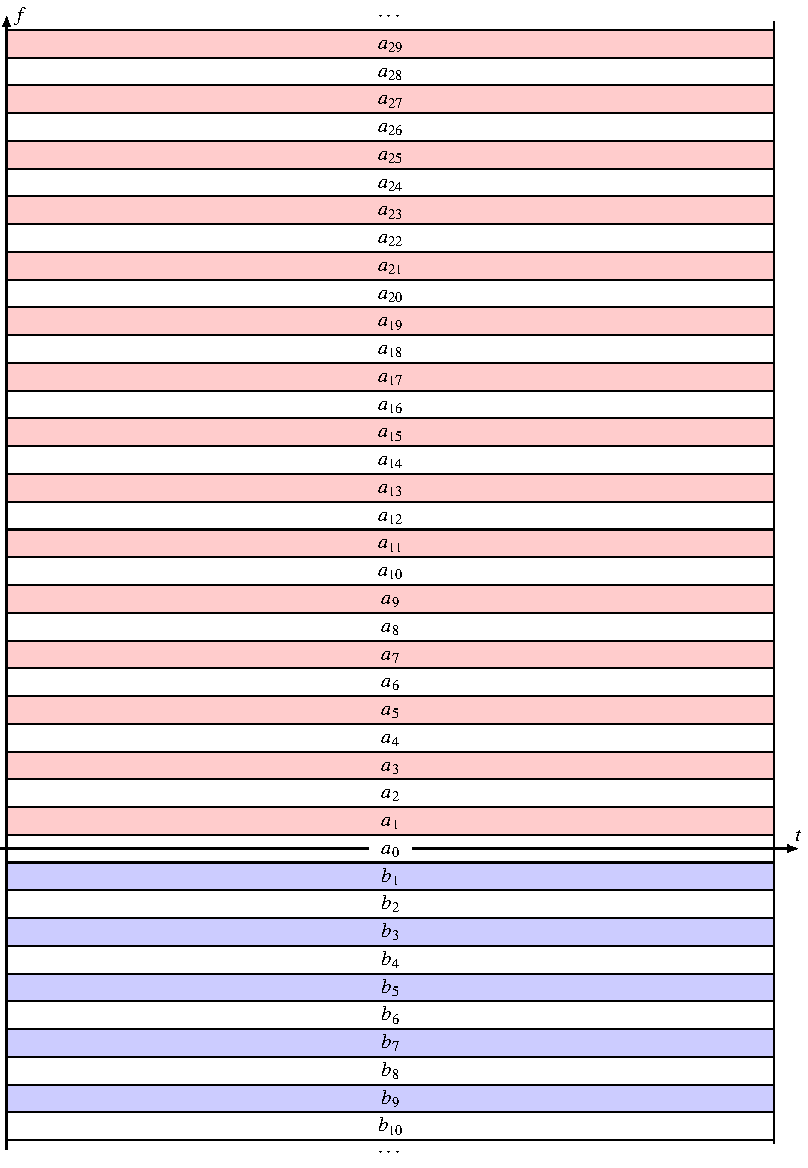
\includegraphics{chapters/2-fourier/images/ft.pdf}
\caption{Aufteilung der Frequenz-Zeit-Ebene für Fourierreihen.
\label{ft:ftplane}}
\end{figure}

Für jedes $k>0$ gibt es daher je einen Koeffizienten $a_k$ und $b_k$,
der das Verhalten des Signals bei der Frequenz $k$ wiedergibt.
Für $k=0$ gibt es genau einen Koeffizienten, nämlich $a_0$, der das
zeitunabhängige Verhalten codiert.
In der Frequenz-Zeit-Ebene lässt sich dieser Sachverhalt wie in 
Abbildung~\ref{ft:ftplane} darstellen.

\subsection{Komplexe Fourier-Reihen}
Eine reelle Funktion in $L^2([0,2\pi])$ lässt sich mit einer Fourier-Reihe
darstellen, deren Koeffizienten alle reell sind.
Für eine komplexe Funktion werden auch die Koeffizienten komplex sein.
Die Form einer reellen Fourier-Reihe ist jetzt nicht mehr unbedingt
vorteilhaft, da die Funktionen $s_k$ und $c_k$ ziemlich unsymmetrisch
sind.
Gesucht ist also eine orthonormiertes Erzeugendensystem aus
$2\pi$-periodischen komplexen Funktionen.
Die Eulersche Gleichung $e^{it} = \cos t + i\sin t$ deutet an, dass
dafür die Funktionen
\[
e_k(t) = e^{ikt}
\]
geeignet sein könnten.
Es ist bereits jetzt klar, dass diese Funktionen ein Erzeugendensystem
bilden, denn es lassen sich daraus mit
\[
\cos kt = \frac{e^{ikt}+e^{-ikt}}2
\qquad\text{und}\qquad
\sin kt = \frac{e^{ikt}-e^{-ikt}}{2i}
\]
alle Funktionen des Erzeugendensystems
der reellen Fourier-Reihen linear kombinieren.
Es bleibt also nur noch sicherzustellen, dass sie auch orthonormiert
sind.
Dazu werden wieder die Skalarprodukte berechnet.
Zunächst gilt für $k\ne l$
\begin{align*}
\langle e_k,e_l\rangle
&=
\int_0^{2\pi} e_k(t) \bar{e}_l(t) \,dt
=
\int_0^{2\pi} e^{ikt}e^{-ilt}\,dt
=
\int_0^{2\pi} e^{i(k-l)t}\,dt
=
\biggl[ \frac{e^{i(k-l)t}}{i(k-l)} \biggr]_0^{2\pi} 
=
0,
\end{align*}
die Funktionen sind also orthogonal.
Sie sind aber nicht normiret, denn für $k=l$ ist 
\[
\|e_k\|^2
=
\int_0^{2\pi} e^{ikt}e^{-ikt}\,dt
=
\int_0^{2\pi} \,dt = 2\pi.
\]
Um die Funktionen zu normieren, muss man also durch $\sqrt{2\pi}$ teilen.

Es folgt also, dass die Funktionen
\[
\mathcal{C}
=
\biggl\{
\frac1{\sqrt{2\pi}} e_k(t)
=
\frac1{\sqrt{2\pi}} e^{ikt}\;\bigg|\; k\in\mathbb Z
\biggr\}
\]
eine Hilbertbasis von $L^2([0,2\pi])$ bilden.
Die Koeffizienten sind 
\[
\tilde{c}_k 
=
\langle f, e_k\rangle
=
\frac1{\sqrt{2\pi}}
\int_0^{2\pi} f(t) e^{-ikt}\,dt
\]
und die zugehörige Reihe ist
\[
f(t)
=
\sum_{k=1} \tilde{c}_k \frac{1}{\sqrt{2\pi}} e^{ikt}.
\]
Wie im Falle der reellen Fourier-Reihe ist es auch bei der komplexen
Fourier-Reihe üblich, die Koffizienten so zusammenzufassen, dass in der
Fourier-Reihe keine Faktoren der Form $1/\sqrt{2\pi}$ nötig sind, also
\[
c_k
=
\frac1{\sqrt{2\pi}} \tilde{c}_k
=
\frac1{2\pi} \int_0^{2\pi} f(t) e^{-ikt}\,dt.
\]
Damit wird die Fourier-Reihe dann
\[
f(t) = \sum_{k\in\mathbb Z} c_k e^{ikt}.
\]

\subsection{Plancherel-Bedingung}
Da die Funktionen $\mathcal{B}$ eine Hilbertbasis bilden, können wir sofort
schliessen, dass die $L^2$-Norm $\|f\|$ einer Funktion $f\in L^2([0,2\pi])$
auch mit den Fourier-Koeffizienten berechnet werden kann.
\[
\| f \|^2
=
|\tilde{a}_0|^2
+
\sum_{k=1}^\infty
(
|\tilde{a}_k|^2
+
|\tilde{b}_k|^2
)
=
\frac{\pi}{2}
|a_0|^2
+
\pi
\sum_{k=1}^\infty
(
|a_k|^2
+
|b_k|^2
)
\]
Dasselbe gilt natürlich auch für die komplexe Fourierreihe.
Dort gilt
\[
\| f\|^2
=
\sum_{k\in\mathbb Z} |\tilde{c}_k|^2
=
2\pi \sum_{k\in\mathbb Z} |c_k|^2.
\]






%
% integral.tex -- Fourier-Integral
%
% (c) 2019 Prof Dr Andreas Müller, Hochschule Rapperswil
%
\section{Fourier-Integral und Fourier-Transformation
\label{section:fourier-integral}}
\rhead{Fourier-Integral}
In $L^2(\mathbb R)$ gibt es ebenfalls eine Transformation, welche
ein Signal im Frequenzbereich analysieren kann.
Da der Definitionsbereich unbegrenzt ist, kann jede beliebige Frequenz
vorkommen.
Die Fourier-Transformation produziert aus einer Funktion $f\in L^2(\mathbb R)$
also eine Funktion $\hat{f}\in\mathbb L^2(\mathbb R)$.

\subsection{Fourier-Integral
\label{subsection:fourier-integral}}
Für Funktionen $f\in L^2(\mathbb R)$ ist die Fourier-Transformation
\[
\hat{f}(\omega)
=
\frac{1}{\sqrt{2\pi}}
\int_{-\infty}^\infty f(t)e^{-i\omega t}\,dt
\]
wohldefiniert.
\index{Fourier-Transformation}
Wir schreiben die Fourier-Transformation auch
\[
\mathcal{F}\colon f\mapsto \hat{f}.
\]
Sie verallgemeinert die Eigenschaften der Fourier-Koeffizienten $c_k$
für Funktionen auf $\mathbb R$.
Für die Rechungen in den folgenden Kapiteln stellen wir hier die
wichtigsen Formeln für die Fourier-Transformation zusammen.

\subsection{Fourier-Umkehrformel
\label{subsection:fourier-umkehrformel}}
Die Fourier-Transformation kann invertiert werden.
\index{Fourier-Umkehrformel}

\begin{satz}
Für $\hat{f}\in L^2(\mathbb R)$ gilt die Umkehrformel
\[
f(t)
=
\frac{1}{\sqrt{2\pi}}
\int_{-\infty}^{\infty} \hat{f}(\omega)e^{i\omega t}\,d\omega.
\]
\end{satz}

Die Fourier-Transformation ist also eine invertierbare lineare Abbildung,
$\mathcal{F}^{-1}\!\left\lbrace\hat{f}\right\rbrace = f$.

\subsection{Translation und Dilatation
\label{subsection:ft-translation-und-dilatation}}
Wenn wir die Fourier-Transformation auf Wavelets anwenden wollen, müssen
wir in der Lage sein, die Fourier-Transformierte von Translaten und
Dilatationen zu berechnen.
Wir berechnen daher die Verträglichkeit von $\mathcal{F}$ mit $T_b$ und
$D_a$ bzw.~$\tilde{D}_a$.

\begin{satz}
\label{four-int:trans-dial}
Die Fourier-Transformation $\mathcal F\colon f\mapsto f$ ist eine linear
Abbildung, die sich mit Translation, Dilatation und Ableitung wie folgt
verträgt:
\begin{align*}
\widehat{T_bf}(\omega)
&=
e^{-i\omega b}\hat{f}(\omega),
\\
\widehat{\tilde{D}_af}(\omega)
&=
a \hat{f}(a\omega)
=
a D_{1/a} \hat{f}(\omega),
\\
\widehat{D_af}(\omega)
&=
D_{1/a}\hat{f}(\omega),
\\
\widehat{e^{ibt}f}(\omega)
&=
(T_b\hat{f})(\omega).
\end{align*}
\end{satz}

\begin{proof}[Beweis]
Durch direkte Rechnung finden wir:
\begin{align*}
\widehat{T_bf}(\omega)
&=
\int_{-\infty}^{\infty} (T_bf)(t)e^{-i\omega t}\,dt
=
\int_{-\infty}^{\infty} f(\underbrace{t-b}_{\displaystyle=t'})e^{-i\omega t}\,dt
=
\int_{-\infty}^{\infty} f(t')e^{-i\omega(t'+b)}\,dt'
\\
&=
e^{-i\omega b}
\int_{-\infty}^{\infty} f(t')e^{-i\omega t'}\,dt'
=
e^{-i\omega b}\hat{f}(\omega).
\\
\widehat{\tilde{D}_af}(\omega)
&=
\int_{-\infty}^\infty (\tilde{D}_af)(t)e^{-i\omega t}\,dt
=
\int_{-\infty}^\infty f(\underbrace{t/a}_{\displaystyle=t'})e^{-i\omega t}\,dt
=
\int_{-\infty}^\infty f(t')e^{-i\omega at'}\,a\,dt'
=
a \hat{f}(a\omega)
\\
\widehat{e^{ibt}f}(\omega)
&=
\int_{-\infty}^\infty e^{ibt}f(t)e^{-i\omega t}\,dt
=
\int_{-\infty}^\infty f(t)e^{-i(\omega -b)t}\,dt
=
\hat{f}(\omega-b)
=
(T_b\hat{f})(\omega).
\end{align*}
Damit sind bis auf die dritte alle Identitäten bewiesen.
Für die dritte wenden wir die Definition $\tilde{D}_a = \sqrt{a}D_a$
auf die zweite Relation an und erhalten
\[
\widehat{D_af}(\omega)
=
\frac{1}{\sqrt{a}}
\widehat{\tilde{D}_af}(\omega)
=
\frac{1}{\sqrt{a}}
a\hat{f}(a\omega)
=
\sqrt{a} \tilde{D}_{1/a}\hat{f}(\omega)
=
D_{1/a}\hat{f}(\omega),
\]
womit auch die dritte Identität bewiesen ist.
\end{proof}

Schreibt man $M_b$ für den Operator, der eine Funktion mit dem
Faktor $e^{ibt}$ multipliziert, also
\[
(M_bf)(t) = e^{ibt}f(t),
\]
dann kann man die Relationen noch etwas kompakter schreiben:
\begin{align*}
\widehat{T_bf}
&=
M_{-b}\hat{f}
\\
\widehat{M_bf}
&=
T_b\hat{f},
\end{align*}
oder mit der Schreibweise $\mathcal{F}f$ für die Fourier-Transformation
\[
\begin{aligned}
\mathcal{F}T_b f &= M_{-b}\mathcal F f
&&\Rightarrow &
\mathcal{F}T_b &= M_{-b}\mathcal{F}
\\
\mathcal{F}M_b f&=T_b\mathcal{F}T_bf
&&\Rightarrow &
\mathcal{F}M_b&=T_b\mathcal{F}T_b
\\
\mathcal{F}\tilde{D}_af&=a \tilde{D}_{1/a} \mathcal F f
&&\Rightarrow &
\mathcal{F}\tilde{D}_a&=a \tilde{D}_{1/a} \mathcal F 
\\
\mathcal{F}D_af&=D_{1/a} \mathcal F f
&&\Rightarrow &
\mathcal{F}D_a&= D_{1/a} \mathcal F 
\end{aligned}
\]

\subsection{Plancherel-Formel}
Die Plancherel-Formel beschreibt, wie sich Skalarprodukt und Norm
unter Fourier-Transformation verhalten.

\begin{satz}
Für zwei Funktionen $f,g\in L^2(\mathbb R)$ gilt die Plancherel-Formel
\begin{align*}
\langle f,g\rangle
&=
\langle \hat{f},\hat{g}\rangle.
\\
\|f\|&=\|\hat{f}\|
\end{align*}
Die Fourier-Transformation $\mathcal{F}\colon f\mapsto \hat{f}$ ist
also eine Isometrie.
\end{satz}

\subsection{Fourier-Transformation und Ableitung
\label{subsection:ft-ableitung}}
Die Ableitung einer Fourier-Transformierten kann direkt berechnet werden.

\begin{satz}
Für differenzierbare Funktionen $f$ gilt
\[
\widehat{f'}(\omega) = i\omega \hat{f}(\omega)
\]
Falls für $g\in L^2(\mathbb R)$ mit $\|tg\|^2<\infty$, dann ist $\hat{g}$
fast überall differenzierbar und es gilt
\[
-\widehat{i t f}(\omega) = \hat{f}'(\omega).
\]
\end{satz}

\begin{proof}[Beweis]
Die Formeln hängen davon ab, ob partiell integiert oder die Ableitung
unter des Integral genommen werden darf:
\begin{align*}
\widehat{f'}(\omega)
&=
\frac{1}{\sqrt{2\pi}}
\int_{-\infty}^\infty \underbrace{f'(t)}_{\uparrow}\underbrace{e^{-i\omega t}}_{\downarrow}\,dt
=
\frac{1}{\sqrt{2\pi}}
\biggl[
f(t)e^{-i\omega t}\,dt
\biggr]_{-\infty}^\infty
+
\frac{1}{\sqrt{2\pi}}
\cdot
i\omega
\int_{-\infty}^\infty f(t)e^{-i\omega t}\,dt
=
i\omega\hat{f}(\omega),
\\
\hat{f}'(\omega)
&=
\frac{d}{d\omega}
\frac{1}{\sqrt{2\pi}} \int_{-\infty}^\infty
f(t) e^{-i\omega t}\,dt
=
\frac{1}{\sqrt{2\pi}} \int_{-\infty}^\infty
-it f(t) e^{-i\omega t}\,dt
=
-\widehat{itf}(\omega)
\qedhere
\end{align*}
\end{proof}

Schreibt man $\partial_t$ für die Ableitung nach $t$ und $\partial_\omega$
für die Ableitung nach $\omega$ und $\mu_{t}$ bzw.~$\mu_{\omega}$ für
die Multiplikation $t$ bzw.~$\omega$, dann kann man die Regeln wieder
kompakter schreiben:
\[
\begin{aligned}
\mathcal{F}\partial_t f &= i\mu_{\omega}\mathcal{F}f
&&\Rightarrow&
\mathcal{F}\partial_t &= i\mu_{\omega}\mathcal{F}
\\
-i\mathcal{F}\mu_t f &= \partial_\omega\mathcal{F} f
&&\Rightarrow&
-i\mathcal{F}\mu_t &= \partial_\omega\mathcal{F}.
\end{aligned}
\]

\subsection{Faltung und Fourier-Transformation
\label{subsection:faltung-und-ft}}

\begin{definition}
\label{definition:faltung}
Die Faltung zweier Funktionen ist
\begin{equation}
(f*g)(t)
=
\int_{-\infty}^\infty f(s)g(t-s)\,ds
\label{definition:formel:faltung}
\end{equation}
\end{definition}
\index{Faltung}
Die Fourier-Transformation verwandelt die Faltung in ein gewöhnliches
Produkt der Fourier-Transformierten:
\begin{align*}
\mathcal{F}(f*g)(\omega)
&=
\frac{1}{\sqrt{2\pi}}
\int_{-\infty}^\infty
f*g(t)
e^{-i\omega t}
\,dt
\\
&=
\frac{1}{\sqrt{2\pi}}
\int_{-\infty}^\infty
\int_{-\infty}^\infty
f(s) g(s-t)
\,ds
\,dt
\\
&=
\frac{1}{\sqrt{2\pi}}
\int_{-\infty}^\infty
\int_{-\infty}^\infty
f(s) g(t-s)
e^{-i\omega s+t-s}
\,ds
\,dt
\\
&=
\frac{1}{\sqrt{2\pi}}
\int_{-\infty}^\infty
f(s) g(\tau)
e^{-i\omega s}
\,ds
\int_{-\infty}^\infty
e^{-i\omega (\tau)}
\,d\tau
\\
&=
\sqrt{2\pi}
\cdot
\underbrace{
\frac{1}{\sqrt{2\pi}}
\int_{-\infty}^\infty
f(s)
e^{-i\omega s}
\,ds}_{\displaystyle \hat{f}(\omega)}
\underbrace{
\frac{1}{\sqrt{2\pi}}
\int_{-\infty}^\infty
g(\tau)
e^{-i\omega (\tau)}
\,d\tau}_{\displaystyle \hat{g}(\omega)}
\\
&=
\sqrt{2\pi}\,
\hat{g}(\omega)\cdot \hat{f}(\omega)
\end{align*}
Wir halten dies im folgenden Satz fest.

\begin{satz}[Faltungsformel]
\label{satz:faltungsformel}
Sind $f,g\in L^2(\mathbb R)$, dann ist die Fourier-Transformierte
der Faltung
\begin{equation}
\widehat{f*g}
=
\sqrt{2\pi}
\hat{f}\cdot \hat{g}
\qquad\text{oder}\qquad
\widehat{f*g}(\omega)
=
\sqrt{2\pi}
\hat{f}(\omega)\, \hat{g}(\omega).
\label{ft:faltungsformel}
\end{equation}
\end{satz}





%
% windowed.tex
%
% (c) 2019 Prof Dr Andreas Müller, Hochschule Rapperswil
%
\section{Gefensterte Fourier-Transformation
\label{section:gefenstert}}
\rhead{Gefensterte Fourier-Transformation}
\begin{figure}
\centering
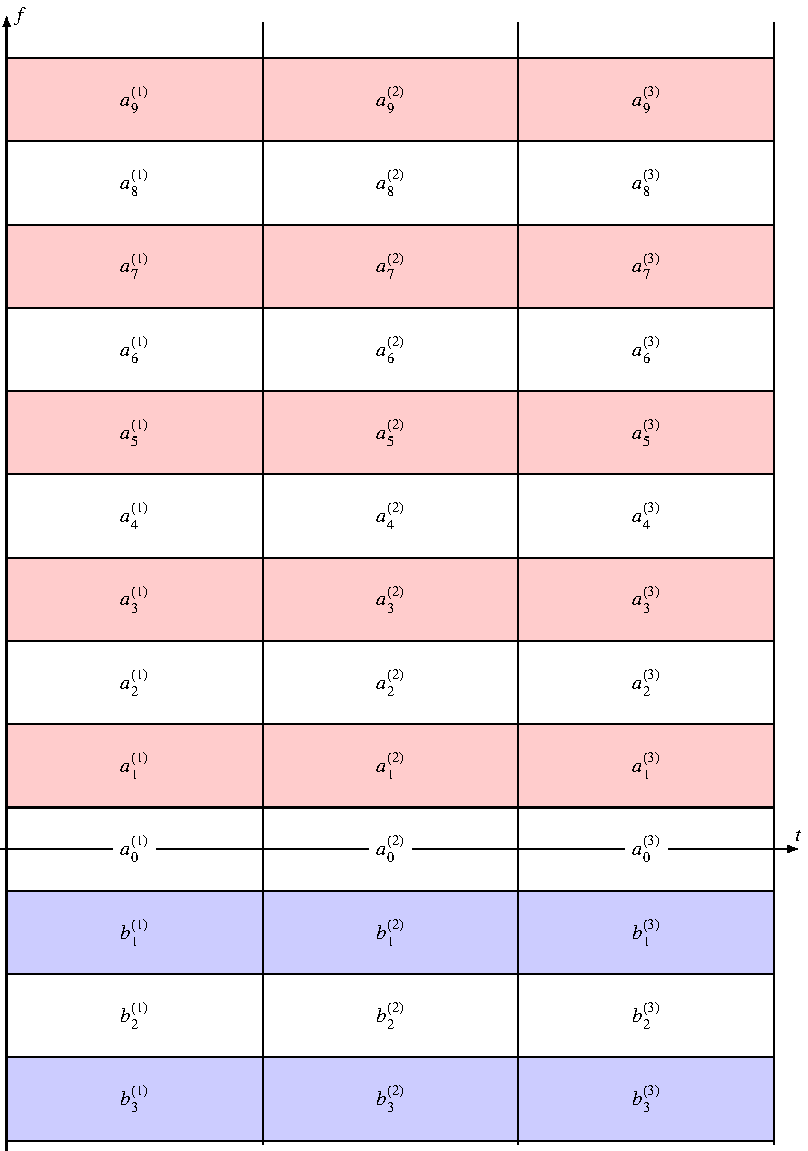
\includegraphics{chapters/2-fourier/images/wft.pdf}
\caption{Aufteilung der Frequenz-Zeit-Ebene für die gefensterte
Fourier-Transformation.
\label{wft:ftplane}}
\end{figure}
Ändert man eine $2\pi$-periodische Funktion in der Umgebung eines Punktes,
dann ändern praktisch alle Fourier-Koeffizienten.
Da die Fourier-Koeffizienten linear von der Funktion abhängen,
reicht es, die Koeffizienten der Änderung zu bestimmen.
Für eine Dirac $\delta$-Distribution im Punkt $t_0$ sind die Koeffizienten
\[
c_k
=
\frac{1}{2\pi} \int_0^{2\pi} \delta(t-t_0) e^{ikt}\,dt
=
\frac{1}{2\pi} e^{ikt_0},
\]
insbesondere ändert jeder Koeffizient um eine Zahl vom Betrag $1/2\pi$.

Die Position einer Störung äussert sich also nur in der Phase, nicht
im Betrag der Störung.
Man könnte sagen, die Information über die Störung ist im Amplitudenspektrum
vollständig delokalisiert.
Diese Eigenschaft der Fourier-Reihen bedeutet, dass transiente Ereignisse
nur sehr beschränkt mit Fourier-Reihen analysiert werden können.

Noch drastischer ist die Situation für die Fourier-Transformation.
Eine $\delta$-Störung in einem Punkt $t_0$ irgendwo auf der reellen Achse
ändert die Transformierte um
\[
\mathcal{\delta_{t_0}}(\omega)
=
\frac{1}{\sqrt{2\pi}} \int_{-\infty}^\infty \delta(t-t_0) e^{-i\omega t}\,dt
=
\frac1{\sqrt{2\pi}} e^{-i\omega t_0}.
\]
Auch in diesem Fall schlägt sich der Ort der Störung nur in der Phase nieder,
nicht in der Amplitude.
Das Amptlitudenspektrum sagt also nichts über die Position der
Störung aus.

Die {\em gefensterte Fouriertransformation} ermöglich, etwas Orts-Information
in die Fourier-Koeffizienten zu rechnen.
Zu diesem Zweck wird das Definitionsgebiet in kleinere Intervalle gleicher
Grösser unterteilt.
In jedem Teil-Intervall kann das vorgegebene Signal in eine Fourier-Reihe
entwickelt werden.
Die so ermittelten Fourier-Koeffizienten können sich dann nur auf den Teil
der Funktion im Teilintervall bezienen.
Eine Störung im Punkt $t_0$ wirkt sich nur auf die Fourier-Koeffizienten
für das Intervall aus, welches $t_0$ enthält.

Die Unterteilung in kleinere Intervalle erhöht aber auch die Frequenz
der Analysefunktionen.
Wird das Intervall $[0,2\pi]$ in $n$ Intervalle unterteilt, dann wird in
jedem Teilintervall mit den Funktionen $e^{inkt}$ für $k\in\mathbb Z$
analysiert.
Die Koeffizienten in den Teilintervallen repräsentieren also ein $n$-mal
grössers Frequenz-Intervall, wie dies in Abbildung~\ref{wft:ftplane}
dargestellt ist.

Die Unterteilung in Teilintervalle löst zwar das Problem der Lokalisierung,
ist aber aus anderen Gründen nicht optimal.
Die Berechnung der Fourier-Reihe für das Teilintervall $[2\pi k/n, 2\pi(k+1)/n]$
läuft darauf hinaus, die Fourier-Reihe im Intervall $[0,2\pi]$ der Funktion
$f(t) \chi_{[2\pi k/n, 2\pi(k+1)/n]}(t)$
zu berechnen, wobei 
\[
\chi_{[2\pi k/n, 2\pi(k+1)/n]}(t)
=
\begin{cases}
1&\qquad t \in [2\pi k/n, 2\pi(k+1)/n]\\
0&\qquad\text{sonst}
\end{cases}
\]
die charakteristische Funktion des Intervalls $[2\pi k/n, 2\pi(k+1)/n]$
ist.
Die Schwierigkeiten rühren daher, dass die charakteristische
Funktion Sprünge aufweist.
Bessere Resultate kann man daher erreichen, wenn man statt einer
charakterisischen Funktion eines Intervalls eine glatte Funktion
verwendet, deren Träger das Intervall enthält.
Die Wahl dieser sogenannten Fensterfunktion beeinflusst die
Analyse-Koeffizienten, bei sorgfältiger Wahl können aber mindestens
die Glattheits-Eigenschaften der analysierten Funktion und die zugehörigen
Eigenschaften der Koeffizienten erhalten werden.

Unbefriedigend bleibt an der gefensterten Fourier-Transformation aber,
dass für jede Frequenz die gleiche Fensterbreite verwendet wird.
Selbst wenn man also zum Beispiel die Sampling-Rate erhöht und damit
die Auflösung verbessert, kann man Transienten in den
Funktionskoeffizienten trotzdem nur mit der Auflösung der Fensterbreite
lokalisieren.
Eine mögliche Verbesserung besteht darin, die Fensterbreite mit zunehmender
Frequenz zu verkleinern.
Genau dies ist, was die Wavelet-Transformation erreicht, die in
Kapitel~\ref{chapter:haar-wavelet} am Beispiel des Haar-Wavelets und in
Kapitel~\ref{chapter:cwt} in voller Allgemeinheit eingeführt wird.


%
% heisenberg.tex
%
% (c) 2019 Prof Dr Andreas Müller, Hochschule Rapperswil
%
\section{Heisenbergsche Unschärfe-Relation
\label{section:heisenberg}}
\rhead{Heisenbergsche Unschärferelation}
Die Fourier-Transformation eines in der Zeit gut lokalisierten
Signals $f(t)$ zeigt, wie gut das selbe Signal im Frequenzraum
lokalisiert ist.
Um diese Idee zu quantifizieren brauchen wir zunächst ein Mass für
die Lokalisierung von $f(t)$ bzw.~$\hat{f}(\omega)$.
Wäre $f$ eine Wahrscheinlichkeitsdichte, dann wäre die Varianz ein
naheliegendes Mass dafür.
Die Funktion muss aber nicht $\le 0$ sein, man könnte das Problem
aber korrigeren, indem man stattdessen $|f(t)|^2$ verwendet.
Das Mass für die Lokalisierung in Zeit und Frequenz ist daher
\begin{align*}
\int_{-\infty}^\infty
t^2 \, |f(t)|^2\,dt
&=
\int_{-\infty}^\infty
|t\,f(t)|^2\,dt
=
\|tf\|^2
\\
\int_{-\infty}^\infty
\omega^2\,|\hat{f}(\omega)|^2\,d\omega
&=
\int_{-\infty}^\infty
|\omega\,\hat{f}(\omega)|^2\,d\omega
=
\|\omega \hat{f}\|^2.
\end{align*}
Je grösser diese Normen werden, desto schlechter ist das Signal in der
entsprechenden Variable lokalisiert.

Die Heisenbergsche Unschärferelation besagt, dass ein Signal nicht
in Zeit und Frequenz gleichzeit beliebig gut lokalisiert sein kann.
Sie drückt dies dadurch aus, dass das Produkt der beiden Normen 
eine untere Schranke hat.

\begin{satz}[Heisenberg]
Ist $f\in L^2(\mathbb R)$ derart, dass 
$\|tf\|<\infty$ und $\|\omega\hat{f}\|<\infty$, dann gilt
\begin{equation}
\| tf \| \cdot \| \omega \hat{f}(\omega)\| \ge \frac12\| f\|^2.
\label{heisenberg:gleichung}
\end{equation}
Die untere Schranke wir erreicht für Gauss-Funktionen, also Funktionen
der Form $De^{-t^2/2\sigma^2}$.
\end{satz}

\begin{proof}[Beweis]
Die Voraussetzungen garantieren, dass die Fourier-Transformation existiert.
Ausserdem bedeutet $\|\omega\hat{f}\|<\infty$, dass $\omega\hat{f}(\omega)$ 
eine $L^2$-Funktion ist.
Nach den Rechenregeln für die Fourier-Transformation besagen, dass 
$f$ fast überall differenzierbar sein muss, enn es gilt
\[
i\omega \hat{f}(\omega) = \widehat {f'}(\omega).
\]
Damit kann man die Lokalisierung von $\hat{f}$ durch $f$ ausdrücken:
\begin{align*}
\|\omega \hat{f}\|^2
&=
\int_{-\infty}^\infty |i\omega \hat{f}(\omega)|^2\,d\omega
=
\int_{-\infty}^\infty |\widehat{f'}(\omega)|^2\,d\omega
\\
&=
\int_{-\infty}^\infty f'(t)|^2\,dt.
\end{align*}
Jetzt kann man die Cauchy-Schwarz-Ungleichung auf die Funktione $f'$ und $tf$
anwenden:
\begin{align*}
\|tf\| \cdot \| f'\|
&\ge
| \operatorname{Re}\langle tf,f'\rangle |
=
\biggl|
\int_{-\infty}^\infty
\frac 12\bigl( tf(t)\bar{f}'(t)  + t\bar{f}(t)f'(t)\biggr)\,dt
\biggr|
\\
&=
\biggl|
\int_{-\infty}^\infty t\cdot \frac{d}{dt}\biggl(\frac12|f(t)|^2\biggr)\,dt
\biggr|
=
\biggl|
\underbrace{
\biggl[
\frac12 t\,|f(t)|^2
\biggr]_{-\infty}^{\infty}
}_{\displaystyle=0}
-
\frac12\underbrace{\int_{-\infty}^\infty |f(t)|^2\,dt}_{\displaystyle=\|f\|^2}
\biggr|
\\
&=
\frac12 \|f\|^2.
\end{align*}
Damit ist die Ungleichung~\eqref{heisenberg:gleichung} bewiesen.

Gleichheit wird erreicht, wenn die beiden Faktoren in der 
Ungleichung~\eqref{heisenberg:gleichung} linear abhängig sein.
Es gibt also einen Proportionalitätsfaktor $c\in\mathbb C$ derart,
dass
\[
\begin{aligned}
&&
tf(t)&=cf'(t)
\\
&\Rightarrow&
\frac{t}{c}&=\frac{d}{dt}\log f(t)
\\
&\Rightarrow&
\frac{t^2}{2c}&=\log f(t) + C
\\
&\Rightarrow&
f(t)&=De^{t^2/2c}.
\end{aligned}
\]
Da die Funktion $f$ in $L^2(\mathbb R)$ sein muss, kommen nur negative
Konstanten $c$ in Frage, wir bezeichnen sie mit $c=-\sigma^2$.
Gleichheit in der Ungleichung~\eqref{heisenberg:gleichung} tritt also
genau dann auf, wenn $f$ die Form
\[
f(t) = D e^{-\frac{t^2}{2\sigma^2}}
\]
hat.
\end{proof}




